\begin{task}{2, Approximating linear vector fields}
For this task, we have two linear vector field datasets, each containing 1000 rows and two columns, for 1000 data points $x_0$ and $x_1$ in two dimensions.\\
Approximating vector fields, associated with a vector to every point in the domain space, can describe the direction and rate of change of the state of the system at all the points. Here we introduce the finite-difference formula 
$$\check{v}^{(k)} =\frac{x_1^{(k)} - x_0^{(k)}}{\Delta t}$$,
$x_0$ means points at time t=0 , and points $x_1$ means points at time t = $\Delta t$, at a short time later.

\textbf{Part one}
we estimate the linear vector field used to generate the points $x_1$ from the points $x_0$. The implementation contains two files \verb|task2.ipynb| are testing results and pictures. \verb|utils.py| is the auxiliary file used to plot output and calculate the trajectory of the point's movement. We use the introduced formula above, we can have the equality as $$v(x_0^{(k)}) = v^{(k)} = Ax_0^{(k)}$$. 
This figure \ref{fig:2.1} shows a visualization of the original dataset distribution.  
\begin{figure}[H]
\centering
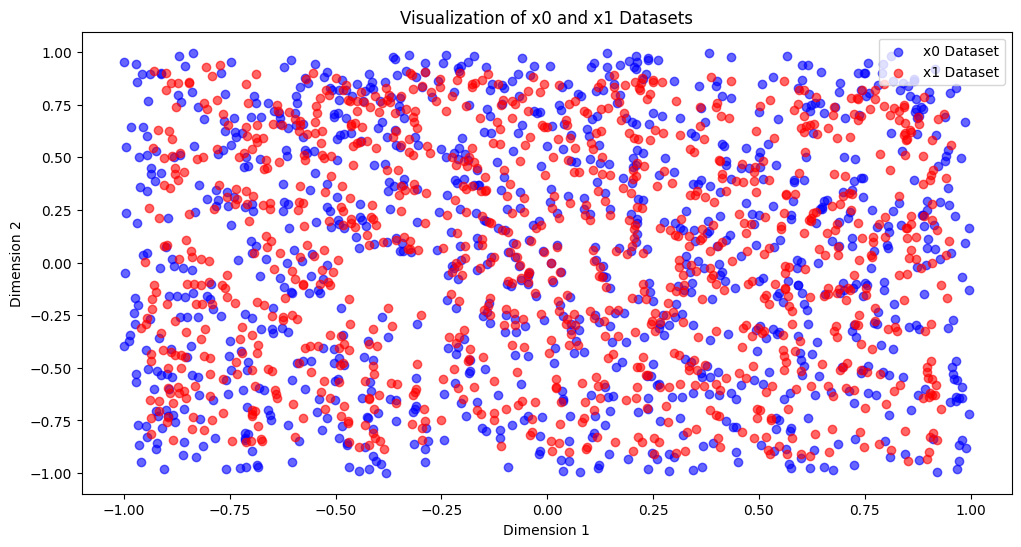
\includegraphics[width=1\textwidth]{images/task2_1.png}
\caption{Initial data distribution}
\label{fig:2.1}
\end{figure}
We are trying to find the optimal coefficient matrix $A \in R^{2x2} $ to represent the mapping relation between these two datasets. After applying the finite difference method, the estimated field vector can be found. We put the estimated field vector into the function \verb|np.linalg.lstsq| the default Numpy function to have estimated coefficient A.

\textbf{Part two}
This task is to solve the linear system and then compute the mean squared error. The estimated A is used to calculate the predicted $x_1$, the implementation function in \verb|utils.py| called trajectory. it will receive the the data position at time t = 0, and the data position after the $\Delta t$ time, also the linear function is also needed. Figure\ref{fig:2.2} showed the trajectory of the after the movement of the delta time. Red dots mean the original poison and green lines are the trajectory of each point. The final result error is $2.83210804e+04$. MSE is 0.32910430761537535. which is quite big in this case. which results in trajectory lines being longer and bigger. 
\begin{figure}[H]
\centering
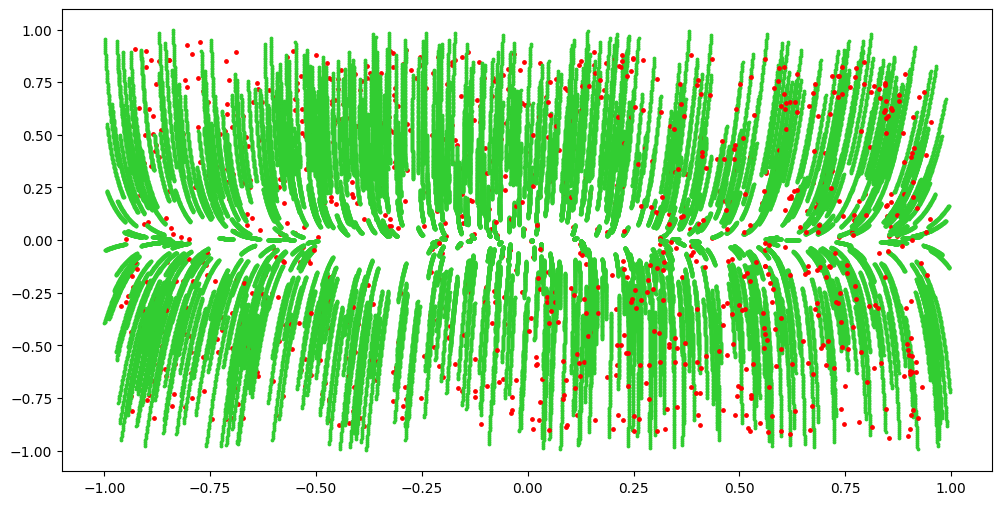
\includegraphics[width=1\textwidth]{images/task2_2.png}
\caption{Trajectory from $x_0$ to $x_1$ with $\Delta t = 0.1$}
\label{fig:2.2}
\end{figure}

\textbf{Part three}
The last part of the task is to visualize the trajectory as well as the phase portrait. \ref{fig:2.3} where you can find the phase portrait of the linear field vector. The direction of each blue line is observed, and the dynamical system looks. The initial point ${10, 10 }$ is set far outside the initial data, we solve this linear system with approximated matrix A, for time $T_{end} = 100 $.  The figure \ref{fig:2.3} demonstrates the dynamic system of all trends from the surrounding area into the middle area which is the reflection of the \ref{fig:2.2} but more clearly. And the orange scatter plot shows the far apart point will reach at the stable state at the end of the time phase. The implementation function is \verb|create_phase_portrait_matrix| in \verb|utils.py|
\begin{figure}[H]
\centering
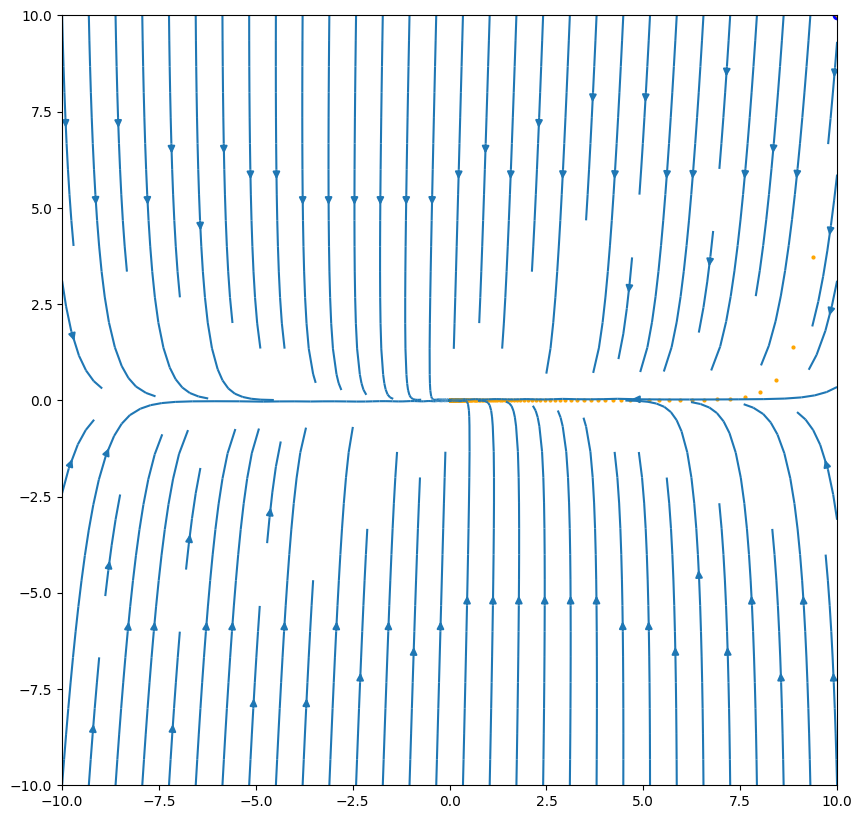
\includegraphics[width=0.6\textwidth]{images/task2_3.png}
\caption{Phase portrait of \(x_0 = [10,10]\) and  \(t_end = 100\)}
\label{fig:2.3}
\end{figure}
\end{task}